% \iffalse
\let\negmedspace\undefined
\let\negthickspace\undefined
\documentclass[journal,12pt,twocolumn]{IEEEtran}
\usepackage{cite}
\usepackage{amsmath,amssymb,amsfonts,amsthm}
\usepackage{algorithmic}
\usepackage{graphicx}
\usepackage{textcomp}
\usepackage{xcolor}
\usepackage{txfonts}
\usepackage{listings}
\usepackage{enumitem}
\usepackage{mathtools}
\usepackage{gensymb}
\usepackage{comment}
\usepackage[breaklinks=true]{hyperref}
\usepackage{tkz-euclide}
\usepackage{listings}
\usepackage{gvv}
\def\inputGnumericTable{}
\usepackage[latin1]{inputenc}
\usepackage{color}
\usepackage{array}
\usepackage{longtable}
\usepackage{calc}
\usepackage{multirow}
\usepackage{hhline}
\usepackage{ifthen}
\usepackage{lscape}

\newtheorem{theorem}{Theorem}[section]
\newtheorem{problem}{Problem}
\newtheorem{proposition}{Proposition}[section]
\newtheorem{lemma}{Lemma}[section]
\newtheorem{corollary}[theorem]{Corollary}
\newtheorem{example}{Example}[section]
\newtheorem{definition}[problem]{Definition}
\newcommand{\BEQA}{\begin{eqnarray}}
\newcommand{\EEQA}{\end{eqnarray}}
\newcommand{\define}{\stackrel{\triangle}{=}}
\theoremstyle{remark}
\newtheorem{rem}{Remark}
\begin{document}

\bibliographystyle{IEEEtran}
\vspace{3cm}

\title{NCERT Discrete 10.5.2 -15}
\author{EE23BTECH11057 - Shakunaveti Sai Sri Ram Varun$^{}$% &lt;-this % stops a space
}
\maketitle
\newpage
\bigskip

\vspace{2cm}
\textbf{Question: }
For what value of $ n$, are the $ nth$ terms of two A.Ps: 63, 65, 67,\dots and 3, 10, 17,\dots equal?\\
\vspace{0.5cm}
\textbf{Solution}:
A sequence is said to be in Arithmetic Progression when it is in the form of
\begin{align}
a, a+d, a+2d, a+3d, \dots
\end{align}
where $a$ is first term and $d$ is common difference.\\
When there are $ n$ terms, the sequence becomes
\begin{align}
a, a+d, a+2d, a+3d,\dots, a+\brak{n}d.\\
T_n = a+\brak{n}d.
\end{align}
which is nth term.
In the given question, there are two sequences.
\begin{align}
63, 65, 67 \dots \label{eq:1}\\
3, 10, 17 \dots \label{eq:2}
\end{align}
let u\brak{n} be unit step function.\\
\begin{align}
u\brak{n} &=
\begin{cases}
1, & if  n \geq 0, \\
0, & if  n < 0.
\end{cases}
\end{align}
\begin{enumerate}
\item
for the sequence $ \eqref{eq:1}$, let x\brak{n} be $ nth$ term, 
\begin{enumerate}
\item
Finding x\brak{n} for sequence $ \eqref{eq:1}$
\begin{align}
a &= 63\\
a+d &= 65\\
\implies x\brak{n} &= 63 + 2n \label{eq:3}\\
\therefore x\brak{n} &= 63u\brak{n} + 2n\cdot u\brak{n}
\end{align}
\item
To find X\brak{z}:
\begin{align}
X\brak{z} &= \sum_{n=-\infty}^{\infty} x\brak{n}\times z^{-n}
\end{align}
\begin{align}
\implies X\brak{z} &= \sum_{n=-\infty}^{\infty} \brak{63u\brak{n}} + 2n\cdot u\brak{n}z^{-n}\\
\implies X\brak{z} &= \sum_{n=0}^{\infty} \brak{63 + 2n}z^{-n}
\end{align}
For the above sum to be convergent:\\
by using ratio test:\\
\begin{align}
    \frac{\brak{n+1}z^{-n-1}}{\brak{n}z^{-n}} &<1\\
   \implies \frac{n+1}{n\cdot z}<1\\
   \therefore |z|>1
\end{align}
This is called region of convergence.\\
\begin{align}
X\brak{z} = \sum_{n=0}^{\infty} \brak{63}z^{-n}+\sum_{n=1}^{\infty}\brak{2n}z^{-n}\\
\implies X\brak{z} = 63z\brak{z-1}^{-1} + 2\brak{2z-1}\brak{z-1}^{-2}\\
\boxed{X\brak{z} = 63z\brak{z-1}^{-1} + 2\brak{2z-1}\brak{z-1}^{-2}}  \forall  |z|>1 \label{eq:5}
\end{align}
\end{enumerate}
\item
for sequence $ \eqref{eq:2}$ , let y\brak{n} be $ nth$ term\\
\begin{enumerate}
\item 
Finding y(n) for $ \eqref{eq:2}$
\begin{align}
a &= 3 \\
a+d &= 10\\
\implies y\brak{n} &= 7n + 3 \label{eq:4}\\
\therefore y\brak{n} &= 3u\brak{n} + 7n\cdot u\brak{n} \label{eq:4}
\end{align}

\begin{figure}[ht]
    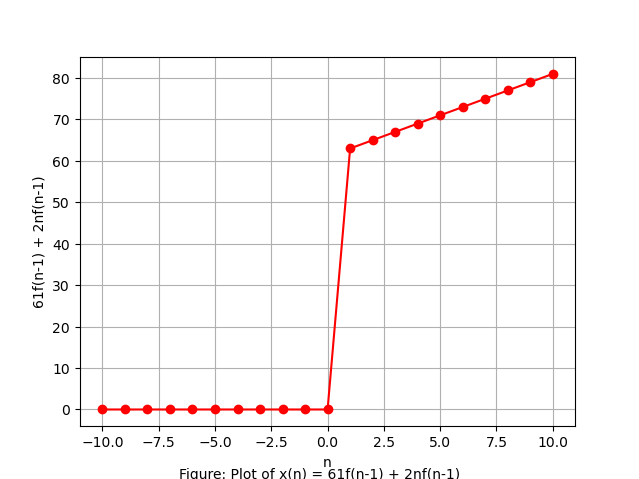
\includegraphics[width = \linewidth]{Figure_1.png}
    \caption{Graphs of x\brak{n}and y\brak{n}}
    \label{Fig:1}
\end{figure}
\item
To find Y\brak{z} :\\
\begin{align}
Y\brak{z} &= \sum_{n=-\infty}^{\infty} y\brak{n}z^{-n}\\
\implies Y\brak{z} &= \sum_{n=-\infty}^{\infty} \brak{3u\brak{n} + 7nu\brak{n}}z^{-n}\\
\implies Y\brak{z} &= \sum_{n=0}^{\infty} \brak{3 + 7n}z^{-n} + 0
\end{align}

even for y(n), R.O.C is $ |z|>1$\\
\begin{align}
Y\brak{z} = \sum_{n=0}^{\infty} \brak{3}z^{-n}+\sum_{n=1}^{\infty}\brak{7n}z^{-n}\\
\implies Y\brak{z} = 3z\brak{z-1}^{-1} + 7\brak{2z-1}\brak{z-1}^{-2}\\
\boxed{Y\brak{z} = 3z\brak{z-1}^{-1} + 7\brak{2z-1}\brak{z-1}^{-2}} \forall  |z|>1 \label{eq:6}
\end{align}
given, x\brak{n} = y\brak{n}\\
\begin{align}
\therefore 63 + 2n &= 7n+3\\
5n &= 60\\
\implies n &= 12
\end{align}
$ \therefore$ 13th terms of given two APs are equal.\\\\
\end{enumerate}
\end{enumerate}


\begin{table}[ht]
    \centering
    \begin{tabular}{|c|c|c|}
    \hline
      variable&description&value\\\hline
         a&first term of an AP&none\\\hline
         x(n)& $ n^{th}$ term of sequence 63,65,67 \dots & 63u\brak{n} + 2nu\brak{n}\\\hline
         y(n)& $ n^{th}$ term of sequence 3,10,17 \dots& 3u\brak{n} + 7nu\brak{n}\\\hline
         X(z)& z-transform of sequence 63,65,67 \dots &$ 63z\brak{z-1}^{-1} + 2\brak{2z-1}\brak{z-1}^{-2}$ \\\hline
         Y(z)& z-transform of sequence 3,10,17 \dots&$ 3z\brak{z-1}^{-1} + 7\brak{2z-1}\brak{z-1}^{-2}$\\\hline
    \end{tabular}
    \caption{parameters used}
    \label{tab:my_label}
\end{table}
\end{document}
